% DESCRIÇÃO DA PROPOSTA--------------------------------------------------------------------


\chapter{INTRODUÇÃO}
\label{chap:introducao}
% Introdução-------------------------------------------------------------------------------
% (máximo de 1 página)
Nos anos recentes, foi notado um grande aumento no tráfego e armazenamento de diferentes aplicações e dados multimídias, como imagens, áudio, vídeo, impressões digitais, séries temporais,
sequências de proteínas, etc. Estes tipos de dados, que apresentam muito mais atributos do que simples numerais ou pequenas cadeias de caracteres, são conhecidos como dados complexos \cite{Zighed2008}.\par
Quando tratados por um Sistema Gerenciador de Banco de Dados Relacional (SGBDR), não suportam comparações com os operadores conhecidos como "big six"\ da linguagem SQL: $=$, $\neq$ , $<$, $>$, $\leq$, $\geq$.
Esse fato limita muito as comparações entre dados complexos inseridos em um SGBDR, ocasionando um grande problema no contexto de base de dados, uma vez que os principais sistemas de gerenciamento
de base de dados são relacionais \cite{DBE2017}. Com isso, tornou-se necessária a concepção de novos tipos de comparadores, como buscas por similaridade.\par 

Estas consultas por similaridade se aplicam de maneira geral a muitos dos tipos de dados complexos \cite{Barioni2009}. Embora equiparar duas imagens médicas (como tomografias de pacientes distintos) 
raramente produza um resultado diferente de falso, procurar por imagens semelhantes à original faz mais sentido e retorna resultados mais relevantes. Dentre os operadores de consulta por similaridade
os mais comuns são as consultas por abrangência (\textit{range query: Rq}) e consulta aos k-vizinhos mais próximos (\textit{k-nearest neighbor querry: kNNq}). As consultas por abrangência \textit{Rq($s_q$, $\xi$)}
recebem como parâmetro um elemento $s_q$ do domínio de dados (elemento central da consulta) e um limite máximo de dissimilaridade $\xi$. O resultado é o conjunto de elementos da base que diferem do elemento
central da consulta por no máximo a dissimilaridade indicada.\par

\begin{figure}[ht]
\centering
\captionsetup{width=0.50\textwidth, font=footnotesize, textfont=bf}
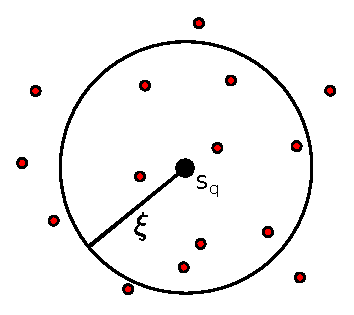
\includegraphics[width=.3\textwidth]{dados/figuras/rq.eps}
\caption{Exemplo de consulta por abrangência}
\label{fig:exemplorq}
\end{figure}


Uma consulta aos k-vizinhos mais próximos \textit{kNNq($s_q$, $k$)} também recebe como um de seus parâmetros um elemento central da consulta $s_q$, e um número inteiro $k$ de vizinhos desejados, e retorna
como resultado o conjunto dos $k$ elementos com a menor dissimilaridade em relação ao elemento central da consulta $s_q$ \cite{POLA2010}. 

Sugere-se fortemente que a  introdução contenha os seguintes itens expressos em parágrafos:

%SGBDR não suporta essas consultas
%Modelo de custo
%SGBDR não possui modelo de custo, impossível de usar técnicas
%OMNI
%B-tree
%várias bases
%extração de métricas e características
%modelagem do problema

P1. Contextualização do Projeto

P2. Definição do Problema

P3. Relevância do Problema

P4. Justificativa

P5. Desafios do Projeto

P6. Contribuição

(substitua este texto pela introdução do trabalho) \\ \\

%-----------------------------------------------------------------------------------------
{\let\clearpage\relax \chapter{OBJETIVOS}}
\label{chap:objetivos}
% (máximo de 1/2 página)

\section{Objetivo Geral}
\label{sec:objgeral}
% Objetivo Geral--------------------------------------------------------------------------
O objetivo geral é tratado em seu sentido mais amplo e constitui a ação que conduzirá ao tratamento da questão abordada no problema de pesquisa, fazendo menção ao objeto de uma forma mais direta. O objetivo geral deve:

Conter descrição do que vai fazer, de forma precisa e objetiva;

Ser diretamente ligado ao título;

Ser mais detalhado que o título;

Resolver o problema proposto;

Ser Claro, Conciso e Completo (CCC) e deve ser verificável ao final do trabalho.

(substitua este texto pelo objetivo geral do trabalho)
%-----------------------------------------------------------------------------------------

\section{Objetivos Específicos}
\label{sec:objespc}
% Objetivos Específicos-------------------------------------------------------------------
Os objetivos específicos apresentam, de forma pormenorizada, detalhada, as ações que se prentede alcançar e estabelecem estreita relação com as particularidades relativas à temática trabalhada. Os objetivos específicos devem:

Ser Claros, Concisos e Completos (CCC) e devem ser verificáveis ao final do trabalho;

Fazem parte do detalhamento do objetivo geral ;

Devem ser iniciados com o verbo no infinitivo;

Podem ser considerados com subprodutos do objetivo geral.

(substitua este texto pelos objetivos específicos do trabalho)

  
%otimização e indexação

%-----------------------------------------------------------------------------------------

% \section{ESTADO DA ARTE}
% \label{sec:estadoarte}
% % Estado da Arte--------------------------------------------------------------------------
% % (máximo de 2 páginas)
% Uma vez formulado o problema a ser atacado, é preciso se inteirar do que já foi feito, dito e discutido sobre ele. Isso se chama "estado da arte". Pode ser que a dúvida, que está motivando a pesquisa, já tenha sido respondida de alguma maneira por alguém. Por isso, é preciso aprofundar o conhecimento sobre a questão, antes de dar prosseguimento ao projeto.
% 
% Essa etapa também recebe o nome de revisão bibliográfica, quando são estudados os trabalhos que se situam na circunvizinhança do problema, trabalhos que versam sobre problemas similares.
% 
% Vê-se aí por que a revisão bibliográfica é importante. De um lado, ela deve comprovar que o pesquisador não está querendo realizar algo que já foi feito, de outro lado, ela ajuda a encaminhar o passo seguinte da pesquisa, a justificativa, quer dizer, a argumentação sobre a relevância do trabalho.
% 
% Para a proposta de TCC deve ser descrito, de maneira breve, alguns (sugestão de 2 (dois) a 3 (três)) trabalhos correlatos, converse com seu orientador para citar os mais relevantes do tema abordado. Pode ser seguido a seguinte sugestão de parágrafos/tópicos:
% 
% P1. Descrição do trabalho 1
% 
% P2. Descrição do trabalho 2
% 
% P3. Descrição do trabalho 3
% 
% P4. Discussão dos trabalhos mencionados destacando porque eles são importantes para o trabalho proposto.
% 
% Para utilização de citações atente ao tipo de citação que se deseja usar. As citações são classificadas em indeireta e direta, podem ser longas ou curtas.
% 
% Uma citação indireta é a transcrição, com suas próprias palavras, das idéias de um autor, mantendo-se o sentido original. A citação indireta é a maneira que o pesquisador tem de ler, compreender e gerar conhecimento a partir do conhecimento de outros autores. Quanto à chamada da referência, ela pode ser feita de duas maneiras distintas, conforme o nome do(s) autor(es) façam parte do seu texto ou não. Exemplo de chamada fazendo parte do texto:\\
% \\Enquanto \citeonline{Maturana2003} defendem uma epistemologia baseada na biologia. Para os autores, é necessário rever \ldots.\\
% 
% A chamada de referência foi feita com o comando \verb|\citeonline{chave}|, que produzirá a formatação correta.
% 
% A segunda forma de fazer uma chamada de referência deve ser utilizada quando se quer evitar uma interrupção na sequência do texto, o que poderia, eventualmente, prejudicar a leitura. Assim, a citação é feita e imediatamente após a obra referenciada deve ser colocada entre parênteses. Porém, neste caso específico, o nome do autor deve vir em caixa alta, seguido do ano da publicação. Exemplo de chamada não fazendo parte do texto:\\
% \\Há defensores da epistemologia baseada na biologia que argumentam em favor da necessidade de \ldots \cite{Maturana2003}.\\
% 
% Nesse caso a chamada de referência deve ser feita com o comando \verb|\cite{chave}|, que produzirá a formatação correta.
% 
% Uma citação direta é a transcrição ou cópia de um parágrafo, de uma frase, de parte dela ou de uma expressão, usando exatamente as mesmas palavras adotadas pelo autor do trabalho consultado.
% 
% Quanto à chamada da referência, ela pode ser feita de qualquer das duas maneiras, assim como nas nas citações indiretas, conforme o nome do(s) autor(es) façam parte do texto ou não. Há duas maneiras distintas de se fazer uma citação direta, conforme o trecho citado seja longo ou curto.
% 
% Quando o trecho citado é longo (4 ou mais linhas) deve-se usar um parágrafo específico para a citação, na forma de um texto recuado (4 cm da margem esquerda), com tamanho de letra menor e espaçamento entrelinhas simples. Exemplo de citação longa:
% \\\begin{citacao}
% Desse modo, opera-se uma ruptura decisiva entre a reflexividade filosófica, isto é a possibilidade do sujeito de pensar e de refletir, e a objetividade científica. Encontramo-nos num ponto em que o conhecimento científico está sem consciência. Sem consciência moral, sem consciência reflexiva e também subjetiva. Cada vez mais o desenvolvimento extraordinário do conhecimento científico vai tornar menos praticável a própria possibilidade de reflexão do sujeito sobre a sua pesquisa \cite[p.~28]{Silva2000}.
% \end{citacao}
% 
% Para fazer a citação longa deve-se utilizar os seguintes comandos:
% \begin{verbatim}
% \begin{citacao}
% <texto da citacao>
% \end{citacao}
% \end{verbatim}
% 
% No exemplo acima, para a chamada da referência o comando \verb|\cite[p.~28]{Silva2000}| foi utilizado, visto que os nomes dos autores não são parte do trecho citado. É necessário também indicar o número da página da obra citada que contém o trecho citado.
% 
% Quando o trecho citado é curto (3 ou menos linhas) ele deve inserido diretamente no texto entre aspas. Exemplos de citação curta:\\
% \\A epistemologia baseada na biologia parte do princípio de que "assumo que não posso fazer referência a entidades independentes de mim para construir meu explicar" \cite[p.~35]{Maturana2003}.\\
% \\A epistemologia baseada na biologia de \citeonline[p.~35]{Maturana2003} parte do princípio de que "assumo que não posso fazer referência a entidades independentes de mim para construir meu explicar".\\
% 
% Outros exemplos de comandos para as chamadas de referências e o resultado produzido por estes são:\\
% \\\citeonline{Maturana2003} \ \ \  \verb|\citeonline{Maturana2003}|\\
% \citeonline{Barbosa2004} \ \ \   \verb|\citeonline{Barbosa2004}|\\
% \cite[p.~28]{Silva2000} \ \ \  \verb|\cite[p.~28]{Silva2000}|\\
% \citeonline[p.~33]{Silva2000} \ \ \   \verb|\citeonline[p.~33]{v}|\\
% \cite[p.~35]{Maturana2003} \ \ \   \verb|\cite[p.~35]{Maturana2003}|\\
% \citeonline[p.~35]{Maturana2003} \ \ \   \verb|\citeonline[p.~35]{Maturana2003}|\\
% \cite{Barbosa2004,Maturana2003} \ \ \   \verb|\cite{Barbosa2004,Maturana2003}|\\
% 
% Em relação as referências, a bibliografia é feita no padrão \textsc{Bib}\TeX{}. As referências são colocadas em um arquivo separado. Neste template as referências são armazenadas no arquivo "base-referencias.bib".
% 
% Existem diversas categorias documentos e materiais componentes da bibliografia. A classe abn\TeX{} define as seguintes categorias (entradas):
% 
% \begin{verbatim}
% @book
% @inbook
% @article
% @phdthesis
% @mastersthesis
% @monography
% @techreport
% @manual
% @proceedings
% @inproceedings
% @journalpart
% @booklet
% @patent
% @unpublished
% @misc
% \end{verbatim}
% 
% Cada categoria (entrada) é formatada pelo pacote \citeonline{abnTeX22014d} de uma forma específica. Para maiores detalhes, refira-se a \citeonline{abnTeX22014d}, \citeonline{abnTeX22014b}, \citeonline{abnTeX22014c}.
%-----------------------------------------------------------------------------------------

{\let\clearpage\relax \chapter{METODOLOGIA}}
% \chapter{METODOLOGIA} % Escolher o nome mais adequado ao trabalho
\label{chap:metodologia}

% Procedimentos Metodológicos/Metodologia-------------------------------------------------
% (máximo de 2 páginas)
Na seção de procedimentos metodológicos ou metodologia (ver qual o nome mais adequado ao trabalho) deve ser descrito sucintamente o procedimentos metodológicos para a execução do projeto ressaltando como os objetivos serão alcançados. 

Em geral, a seção descreve os procedimentos usados para resolver o problema atacado. Pode ser estruturada em tópicos, onde cada tópico representa um subproduto do objetivo geral.

No caso de desenvolvimento de sistemas deve-se descrever a metodologia a ser utilizada, por exemplo Scrum, eXtreme Programming, RUP, etc. 

Também pode ser descritos técnicas de desenvolvimento de software como por exemplo TDD, BDD, SPA,  etc.

(substitua este texto pelo de procedimentos metodológicos/metodologia do trabalho)
%-----------------------------------------------------------------------------------------

\section{MATERIAIS}
\label{sec:materiais}
% Recursos Necessários--------------------------------------------------------------------
Coloque todos os materiais que serão utilizados. Exemplos: computadores, equipamentos de redes, licenças de software, etc. Também deverá ser colocado se os recursos estarão disponíveis. A universidade não comprará os recursos, portanto a responsabilidade de comprar algo será do aluno. (substitua este texto pelo de recursos necessários do trabalho)
%--------

\section{METODOS}
\label{sec:metodos}
Aqui entram os métodos envolvidos no trabalho. \\ \\



 
{\let\clearpage\relax \chapter{CONCLUSÃO}} % Escolher o nome mais adequado ao trabalho
\label{chap:conclusao}
% Conclusão/Considerações Finais----------------------------------------------------------
% (máximo de ½ página)
Na seção de Conclusão ou Considerações Finais (ver qual o nome mais adequado ao trabalho) o acadêmico deve descrever:

Como espera alcançar os objetivos propostos;

Destacar as dificuldades encontradas e previstas;

Fazer o fechamento do trabalho destacando sua importância.

(substitua este texto pelo de estado da arte do trabalho)
%Viabilidade
%-----------------------------------------------------------------------------------------
 \\ \\
 
 
{\let\clearpage\relax \chapter{CRONOGRAMA}}
\label{chap:cronograma}

%Estudo, modelagem, verificação das estruturas OMNI, bases, extratores, métricas, criar o banco e inserir as métricas, implementação da OMNI, implementação seq sem OMNI, comparação
% Planejamento do Trabalho----------------------------------------------------------------
% Esta seção não precisa ser editada, apenas edite o quadro 1 armazenada no diretório ".\dados\quadros"
O planejamento do trabalho de estágio que será desenvolvido pelo aluno, ao longo do período letivo, está descrito no cronograma da Quadro 1. Neste cronograma constam todas as atividades com seus respectivos prazos para o cumprimento.
\begin{quadro}[!htb]
    %\centering
    \caption{Cronograma de Atividades.\label{qua:cronograma}}
    \begin{tabular}{|p{5.0cm}|p{0.6cm}|p{0.6cm}|p{0.6cm}|p{0.6cm}|p{0.6cm}|p{0.6cm}|p{0.6cm}|p{0.6cm}|p{0.6cm}|p{0.6cm}|}
        \hline
        \textbf{Atividades} 						     & 	   \textbf{Set}      & \textbf{Out} & \textbf{Nov} & \textbf{Dez} & \textbf{Jan} & \textbf{Fev} & \textbf{Mar} & \textbf{Abr} & \textbf{Mai} & \textbf{Jun} \\
        \hline
        \footnotesize{1. Estudo e acompanhamento da literatura}		     & X	             & X            &  		   & 		  &  		 &   	        &   	       &   	      & 	     & 		     \\
        \hline
        \footnotesize{2. Modelagem do problema} 				     & X	             & X            &  		   & 		  &  		 &   	        &   	       &   	      & 	     &                \\
        \hline
	\footnotesize{3. Verificação das estruturas Omni} 			     &  	             & X            & X		   & 		  &  		 &   	        &   	       &   	      & 	     &                \\
        \hline
	\footnotesize{4. Estudo dos extratores de características} 		     &  	             &              & X		   & 		  &  		 &   	        &   	       &   	      & 	     & 		     \\
        \hline
	\footnotesize{5. Estudo e inserção das métricas no banco} 		     &  	             & X            & X		   &  		  &  		 &   	        &   	       &   	      & 	     & 		     \\
        \hline
	\footnotesize{6. Criação e povoamento da base de dados} 		     &  	             &              & X		   & X		  &  		 &   	        &   	       &   	      & 	     & 		     \\
        \hline
        \footnotesize{7. Elaboração da apresentação do TCC1}			     &  	             &              & X		   & X		  &  		 &   	        &   	       &   	      & 	     & 		     \\
        \hline        
        \footnotesize{8. Defesa do TCC1}                                             &  	             &              &  		   & X		  &  		 &   	        &   	       &   	      & 	     & 		     \\
        \hline
	\footnotesize{9. Implementação da busca sequencial} 			     &  	             &              &  		   & 		  & X		 & X	        & X 	       &   	      & 	     & 		     \\
        \hline
        \footnotesize{10. Implementação da técnica Omni} 			     &  	             &              &  		   & 		  & X		 & X 	        & X 	       &   	      & 	     & 		     \\
        \hline
        \footnotesize{11. Comparação e análise de resultados} 			     &  	             &              &  		   & 		  &  		 &   	        &  X	       & X 	      & 	     & 		     \\
        \hline
        \footnotesize{12. Implementação da interface} 				     &  	             &              &  		   & 		  &  		 &   	        &  X	       &  X	      & 	     & 		     \\
        \hline
        \footnotesize{13. Elaboração da apresentação final} 			     &  	             &              &  		   & 		  &  		 &   	        &   	       &  X	      &  X	     & 		     \\
        \hline        
        \footnotesize{14. Defesa do TCC2}					     &  	             &              &  		   & 		  &  		 &   	        &   	       &   	      & 	     & X	     \\
        \hline
    \end{tabular}
\end{quadro}

%Estudo, modelagem, verificação das estruturas Omni, bases, extratores, métricas, criar o banco e inserir as métricas, implementação da Omni, implementação seq sem Omni, comparação
%-----------------------------------------------------------------------------------------
